\documentclass[landscape]{article}
\usepackage{wallpaper}
\usepackage{niceframe}
\usepackage{xcolor}
\usepackage{ulem}
\usepackage{graphicx}
\usepackage{geometry}
\geometry{tmargin=.75cm,bmargin=.25cm,lmargin=.8cm,rmargin=.2cm}
\usepackage{multicol}

\begin{document}
%%%%%%%%%%%
\centering
\scalebox{3}{\color{green!30!black!60
\begin{minipage}{.33\textwidth}
\font\border=umrandb
\generalframe
{\border \char113} % up left
{\border \char109} % up
{\border \char112} % up right
{\border \char108} % left
{\border \char110} % right
{\border \char114} % lower left
{\border \char111} % bottom
{\border \char115} % lower right
{\centering

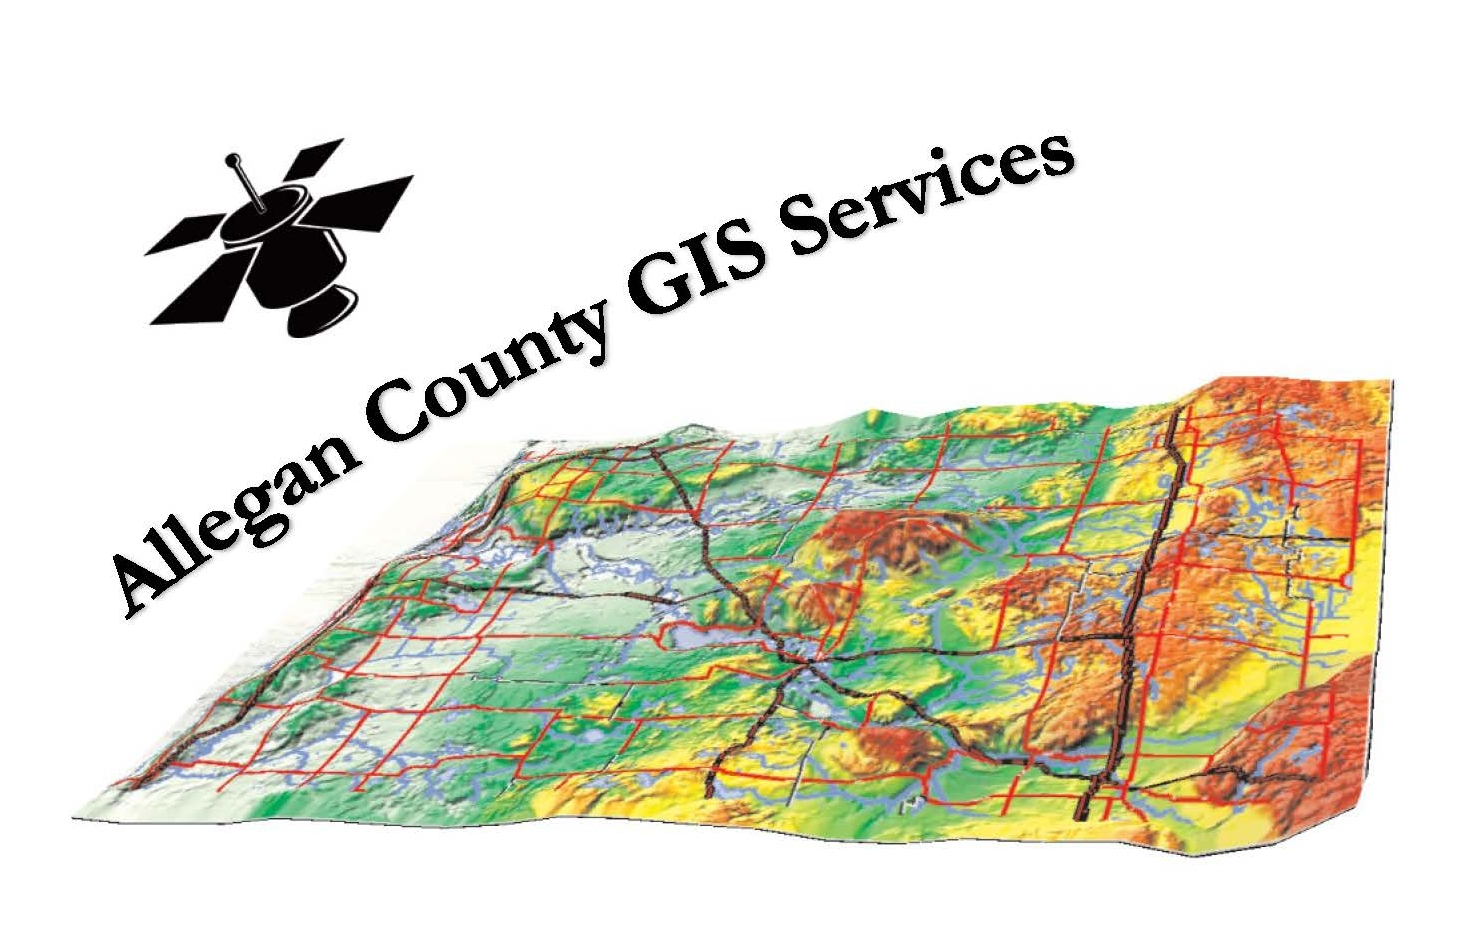
\includegraphics[height=1.25cm]{GIS_Logo_better.jpg}}
\end{minipage}
}}
\vspace{-8mm}
%%%%%%%%%%
\curlyframe[.9\columnwidth]{

\textcolor{red!10!black!90}
{\small Allegan County GIS Services}\\
\textcolor{green!10!black!90}{
\tiny recognizes}

\\
\uline{\textcolor{black}
{Ian Hanes}}
\\
\smallskip
\tiny Chief Equalization Technician
\smallskip

\textcolor{green!10!black!90}
{
\tiny as a
}
\smallskip
\tiny
\\
\textcolor{black}{\large \textsc{GIS Champion}}
\\
\vspace{1mm}
\textcolor{green!10!black!90}
{
\tiny for outstanding dedication and service to the community
\\while using GIS technology on this day
\itshape June 29, 2018
}
\vspace{3mm}

{\color{blue!40!black}
\scalebox{.6}{
\begin{tabular}{ccc}
\cline{1-1}
%\cline{2-2}
\cline{3-3}
%\cline{4-4}
%\cline{5-5}
\\
Neil Besteman  & &  Bryan May \\
GIS Manager & & GIS Analyst \\
\end{tabular}
}}}
\end{document}